\documentclass{beamer}
\usepackage{graphicx}
\usepackage{amsmath}
\usepackage{amsfonts}
% Import listings for code representation
%\usepackage{listings}
%\usepackage{color}
%\usepackage{xcolor}
%% \usepackage{fancyhdr}
%
%\definecolor{mygreen}{rgb}{0,0.6,0}
%\definecolor{mygray}{rgb}{0.5,0.5,0.5}
%\definecolor{mymauve}{rgb}{0.58,0,0.82}
%\lstset
%  {backgroundcolor=\color{white},  % choose the background color; you must add \usepackage{color} or \usepackage{xcolor}; should come as last argument
%  basicstyle=\footnotesize\ttfamily,        % the size of the fonts that are used for the code
%  breakatwhitespace=false,         % sets if automatic breaks should only happen at whitespace
%  breaklines=true,                 % sets automatic line breaking
%  captionpos=b,                    % sets the caption-position to bottom
%  commentstyle=\color{mygreen},    % comment style
%  deletekeywords={},               % if you want to delete keywords from the given language
%  escapeinside={\%*}{*)},          % if you want to add LaTeX within your code
%  extendedchars=true,              % lets you use non-ASCII characters; for 8-bits encodings only, does not work with UTF-8
%  firstnumber=1,                   % start line enumeration with line 1000
%  frame=single,                    % adds a frame around the code
%  keepspaces=true,                 % keeps spaces in text, useful for keeping indentation of code (possibly needs columns=flexible)
%  keywordstyle=\color{blue},       % keyword style
%  language=c++,                    % the language of the code
%  morekeywords={},                 % if you want to add more keywords to the set
%  numbers=left,                    % where to put the line-numbers; possible values are (none, left, right)
%  numbersep=5pt,                   % how far the line-numbers are from the code
%  numberstyle=\tiny\color{mygray}, % the style that is used for the line-numbers
%  rulecolor=\color{black},         % if not set, the frame-color may be changed on line-breaks within not-black text (e.g. comments (green here))
%  showspaces=false,                % show spaces everywhere adding particular underscores; it overrides 'showstringspaces'
%  showstringspaces=false,          % underline spaces within strings only
%  showtabs=false,                  % show tabs within strings adding particular underscores
%  stepnumber=2,                    % the step between two line-numbers. If it's 1, each line will be numbered
%  stringstyle=\color{mymauve},     % string literal style
%  tabsize=2,                       % sets default tabsize to 2 spaces
%  title=\lstname,                  % show the filename of files included with \lstinputlisting; also try caption instead of title
%}

% Import these packages for drawing markov chains
\usepackage{tikz}
\usetikzlibrary{automata, positioning}
\usepackage[most]{tcolorbox}

%\usepackage{hyperref}
%\hypersetup{colorlinks=false, linkcolor=blue, urlcolor=blue,}
%\usepackage{setspace}
%\usepackage{multicol}

% \usepackage{changepage} % For changing the margin of parts of the page
%\usepackage[section]{placeins} % don't allow figures to overflow to other sections

% xepersian should be the last package that is loaded
\usefonttheme{serif}
\usepackage[localise=on]{xepersian}
\settextfont{XB Niloofar}
% \settextfont{BNazanin}
\setlatintextfont{Crimson}
% Fonts
%\settextfont[Scale=1.1]{B Nazanin}
%\setlatintextfont{Times New Roman}

\beamertemplatenavigationsymbolsempty
\usetheme{CambridgeUS}
%\usecolortheme{beaver}
\useoutertheme{miniframes}
%\useinnertheme{circles}
% ------------------------------------------------------------------------------

% Title Definition
\def \mytitletextfa {بهینه‌سازی توزیع‌بار برای سکو‌های خدمات پردازش بدون‌میزبان با استفاده از روش‌های مدل‌سازی}
\def \mytitletexteng {‫‪Optimizing Load Balancing for Serverless Computing Platforms Using Modeling Approaches}
\def \myauthorname {فربد شاهین‌فر}
\def \mystdno{۹۹۲۰۱۴۷۶}
\def \myuniversity{دانشگاه صنعتی شریف}
\def \mydepartment{دانشکده مهندسی کامپیوتر}
\def \mymajro{مهندسی نرم‌افزار}
\def \mylogo{res/logo.pdf}  % نشان دانشگاه
\def \advisorname{دکتر علی موقر رحیم‌آبادی}
\def \adversaryname{دکتر جعفر حبیبی}
\def \mydatetext{بهمن ۱۴۰۰}

% ------------------------------------------------------------------------------
\newcommand{\mytitle}{
	\centering
	% Logo
	\begin{flushright}
	\begin{tabular}{cc}
		\centering
		\includegraphics[width=0.1\linewidth]{\mylogo} &
		\raisebox{0.03\linewidth}
		{\begin{tabular}{r}
				\tiny\myuniversity \\
				\tiny\mydepartment \\
				{\tiny سمینار کارشناسی ارشد گرایش \mymajro}
		\end{tabular}}
	\end{tabular}
	\end{flushright}
% 	\begin{figure}[!h]
%	   	\centering
%		 \includegraphics[width=0.12\linewidth]{\mylogo}
%	\end{figure}
%	{\tiny \myuniversity \\ \mydepartment \\ \raisebox{2mm}{سمینار کارشناسی ارشد گرایش \mymajro}}
	\vspace{0.5cm}
	\begin{center}
 	 % Title
	 {\textbf{\mytitletextfa} \\ \vspace{3mm} \latin{\textbf{\mytitletexteng}}}

  % Author information
  \vspace{3mm}
  {\small  نگارش: {\myauthorname} - {{\mystdno}} \par}
  \vspace {3mm}
  {\small استاد راهنما: {\advisorname}\par}
  \vspace {3mm}
  {\small استاد ممتحن داخلی: {\adversaryname} \par}
  % Date
  \vspace {0.5cm} {\small\mydatetext\par}
	\end{center}
}

%\renewcommand{\sectionmark}[1]{\markboth{#1}{}}
%\pagestyle{fancy}
%\rhead{}
%\chead{}
%\lhead{\leftmark}

% Command Definitions
\newcommand{\myhline}{\noindent\rule[0.5ex]{\linewidth}{1pt}\par}
\newcommand{\زیرل}[1]{\footnote{\lr{#1}}}
\def\مل{\lr}
\makeatletter
\newcommand{\RTList}{\raggedleft\rightskip\@totalleftmargin} 
\makeatother
\newcommand{\توچشم}[1]{\textit{\color{blue}#1}}
\newcommand{\mybox}[2]{\begin{minipage}{0.8\linewidth}
	\setbeamertemplate{block begin}[default]
	\setbeamertemplate{block end}[default]
	\begin{block}{#1}
		#2
	\end{block}
\end{minipage}}
% ------------------------------------------------------------------------------

% Document Specific Definitions
\def\cpu{N_{cpu}}
% ------------------------------------------------------------------------------

\begin{document}
\begin{persian}
\everypar{\rightskip\rightmargin}

% Title page
\begin{frame}
	\mytitle
\end{frame}
% Tables
%\begin{frame}{فهرست مطالب}
%	% Why aligning this to the right was so hard?
%	\begin{flushright}
%	\hspace{1cm}
%	\begin{minipage}{5cm}
%		\tableofcontents[hideallsubsections]
%	\end{minipage}
%	\end{flushright}
%\end{frame}
% Show list of things in beging of each section
\AtBeginSection[ ]
{
\begin{frame}{فهرست مطالب}
	\begin{flushright}
		\hspace{1cm}
		\begin{minipage}{10cm}
			\tableofcontents[currentsection]
		\end{minipage}
	\end{flushright}
\end{frame}
}

% Goal
\begin{frame}{هدف}
	\begin{itemize}\RTList
	\فقره پردازش بدون‌میزبان راهکار جدیدی برای ارائه خدمات ابری است.
	\فقره توزیع مناسب بار کاری یکی از بخش‌های اساسی آن است. 
	\فقره هدف از این پروژه ارزیابی کارایی الگوریتم‌های توزیع‌بار مودجود برای سکوهای پردازش بدون‌میزبان است.
	\فقره ایجاد یک مدل مناسب از این سیستم امکان تحلیل مناسب را ایجاد می‌کند.
	\end{itemize}
\end{frame}

%% Abstract
%\قسمت*{چکیده}
\markboth{چکیده}{}

پردازش بدون‌میزبان تحولی در پردازش ابری است و فرصت‌ها و چالش‌های فراوانی
را به وجود آورده است. مقیاس‌پذیری و اتکاپذیری رکن اساسی این رویکرد است که
از طریق زیر سیستم همنوازی موجود در سکو‌های ارائه خدمات به تحقق می‌پیوندد.
توزیع‌بار بخشی از زیر سیستم همنوازی است که امکان اعمال سیاست‌های مورد نظر را
برای انتخاب زمان پردازش درخواست و خدمت‌گزار مناسب فراهم می‌آورد.
از این روی فهم نحوه عملکرد سیاست‌های توزیع‌بار اهمیت دارد. در این پروژه با استفاده
از روش‌های مدل‌سازی و شبیه‌سازی اقدام به بررسی الگوریتم‌های توزیع‌بار می‌گردد
و با توجه به نتایج مقایسات یک الگوریتم توزیع‌بار جدید ارائه می‌شود.

\متن‌سیاه{واژه‌های کلیدی:}
‫پردازش بدون‌میزبان، پردازش ابری، توزیع با، شبکه‌های مراکز داده، مدل سازی کارایی سیستم‌های کامپیوتری
% Preliminaries
\section{مقدمه}

%\begin{frame}{پردازش ابری}
%	تعریف پردازش ابری ...
%\end{frame}

\begin{frame}{اهمیت پردازش ابری}

ارائه خدمات ابری باعث رشد پیشرفت در علم و صنعت شده است.

\begin{itemize}\RTList
\فقره \مل{CERN} به کمک خدمات ابری گوگل چندین پتابایت داده را در سال پردازش می‌کند\مرجع{google_cern}.
\فقره تمام زیرساخت \مل{Netflix} از خدمات آمازون است\مرجع{amazon_netflix}.
\فقره شرکت \مل{Micros} از خدمات آمازون برای پویانمایی فیلم‌ها استفاده می‌کند\مرجع{amazon_mikros}.
\end{itemize}
\end{frame}

\begin{frame}{ویژگی پردازش ابری}
	در خدمات ابری دو مورد زیر اهمیت بسزایی دارند.
	\begin{itemize}\RTList
		\فقره مقایس‌پذیری
		\فقره اتکاپذیری
	\end{itemize}
	\pause
	\begin{center}
		\mybox{راهکار}{
	استفاده از معماری‌های توزیع‌شده مانند \توچشم{میکروسرویس} راهکار مورد استفاده
	در عمل برای رسیدن به این دو مورد است\مرجع{baboi2019dynamic}.	}		
	\end{center}
\end{frame}

\begin{frame}{معماری میکروسرویس}
	\begin{itemize}\RTList
	\فقره در این معماری، سیستم به مولفه‌هایی ریزدانه‌ و مستقل تقسیم می‌شود.
	\فقره موله‌ها با یک دیگر در بستر شبکه‌های کامپیوتری در ارتباط هستند.
	\فقره هر مولفه می‌توانند به صورت جداگانه بر روی تعدادی خدمت‌رسان اجرا شود.
	
	\pause
	\begin{itemize}\RTList
		\فقره درصورت نیاز به توان پردازشی یک مولفه می‌توان تعداد خدمت‌رسان‌های آن را افزایش داد.
		\فقره درصورت کاهش بار کاری می‌تواند تعداد خدمت‌رسان‌ها را کاهش داد تا در هزینه صرفه‌جوی شود.
		\فقره درصورت رخدادن اشکال برای یک خدمت‌گزار، دیگر خدمت‌گزار‌ها می‌تواند پردازش را ادامه دهند.
	\end{itemize}
	\end{itemize}
\end{frame}

\begin{frame}{مثالی از یک معماری میکروسرویس}
	\begin{figure}
		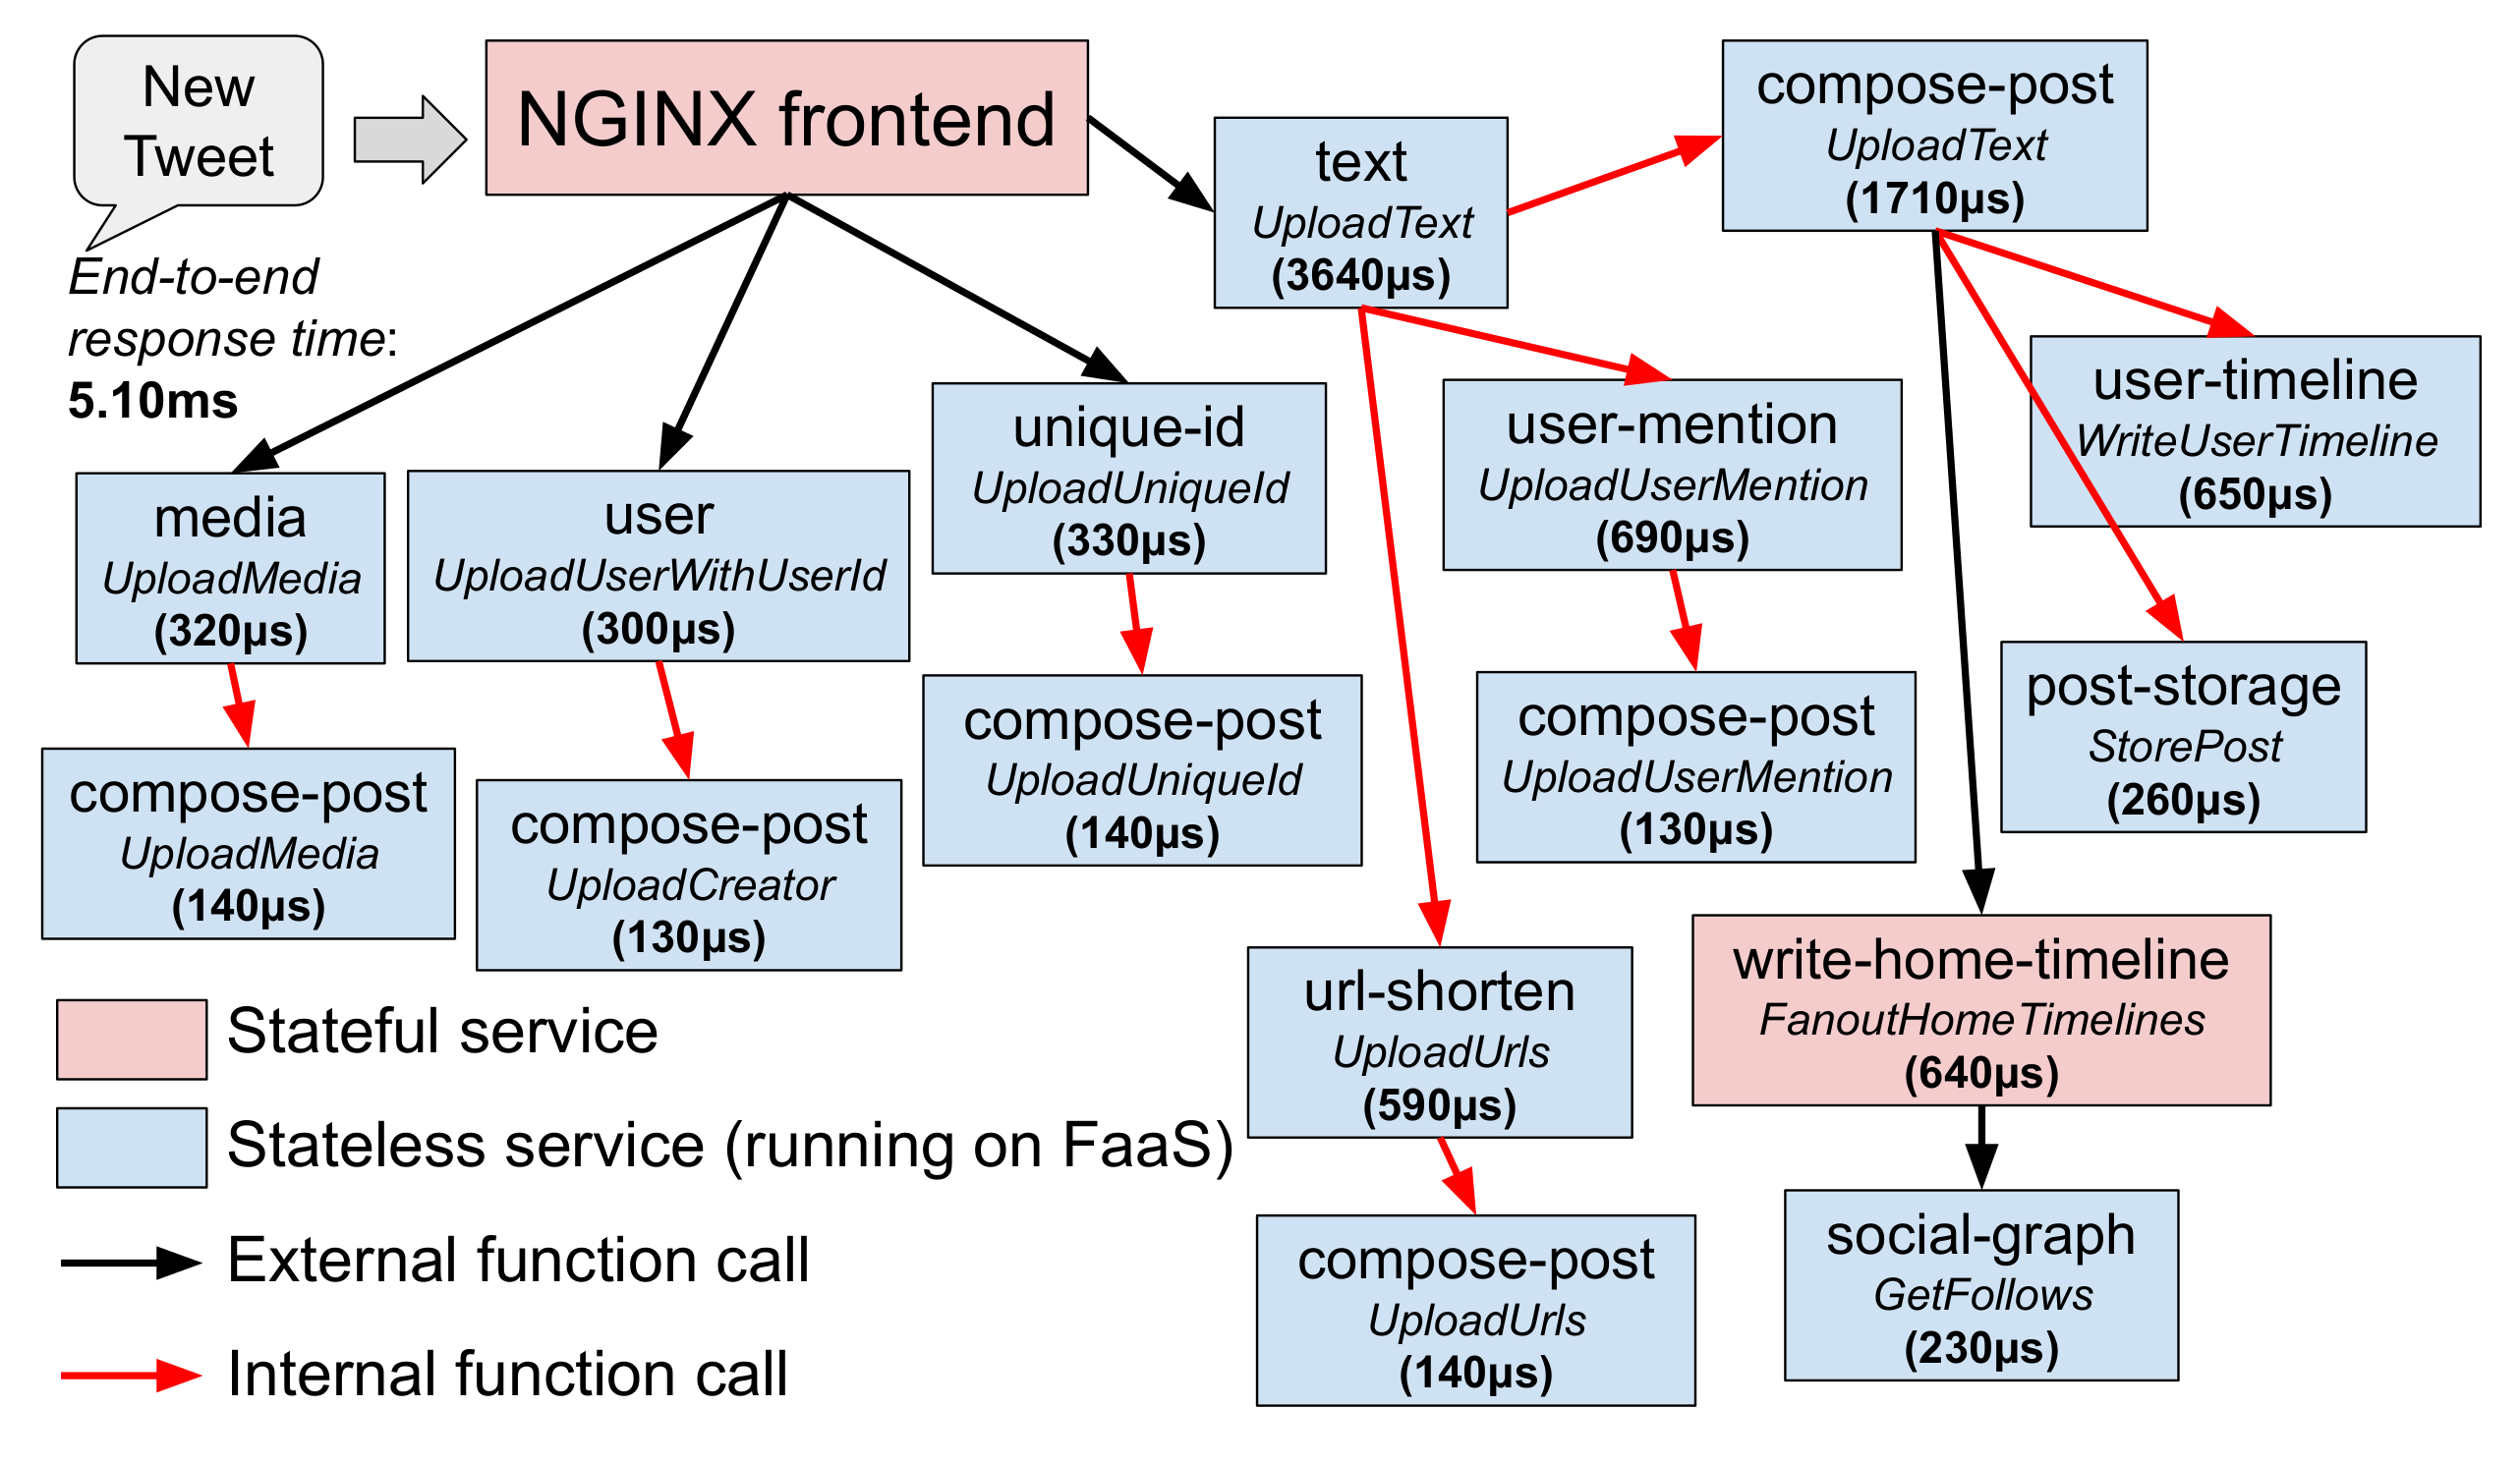
\includegraphics[width=0.8\linewidth]{res/tweet_microservice.png}
		\شرح{مثالی از زنجیره مولفه برای ارسال یک توویت (برگرفته از \مرجع{jia2021nightcore})}
	\end{figure}
\end{frame}

\begin{frame}{نیاز به توزیع‌کننده بار}
	\begin{itemize}\RTList
	\فقره در این معمار چندین خدمت‌گزار یک مولفه یکسان را اجرا می‌کنند.
	\فقره توزیع‌کننده بار تصمیم می‌گیرد که درخواست‌ها در کدام خدمت‌رسان پردازش شوند.
	\فقره هدف این است که دریافت کننده خدمات چندین خدمت‌گزار به صورت یک خدمت‌گزار مشاهده کند.
	\end{itemize}
	\begin{figure}
		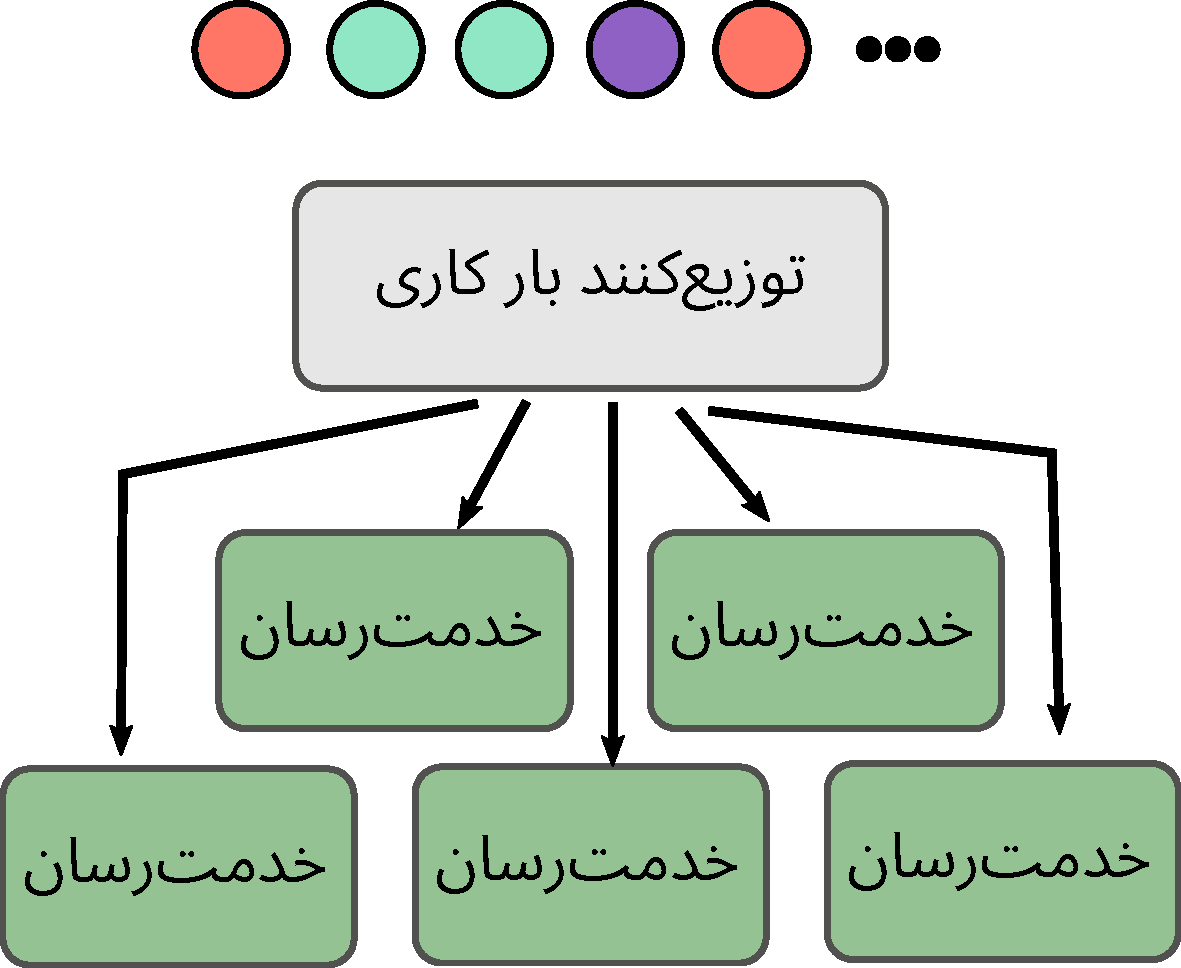
\includegraphics[width=0.4\linewidth]{res/loadbalancer.pdf}
	\end{figure}
\end{frame}

\begin{frame}{پیچیدگی زیرساخت معماری میکروسرویس}
	\mybox{چالش}{
		ایجاد و پیاده‌سازی سیستم‌های نرم‌افزاری با ویژگی‌های شرح داده شده هزینه‌بر و دارای
		چالش‌های فنی بسیاری است.
	}
\end{frame}

\begin{frame}{خدمات پردازش بدون‌میزبان}
	\begin{itemize}\RTList
	\فقره پردازش بدون‌میزبان یک چارچوب پردازش ابری است.
	
	\فقره برنامه ساز می‌تواند برنامه خود را بدون
	نیاز به فعالیت‌های اجرایی مانند تهیه و تخصیص منابع پردازشی ایجاد و اجرا کند.
	
	\فقره وظیفه مسائل مربوط به \توچشم{اتکاپذیری} و \توچشم{مقیاس‌پذیری} بر عهده ارائه دهنده خدمات است. 
	
	\فقره میزان هزینه این خدمات بر اساس
	میزان مصرف واقعی برنامه از منابع موجود محاسبه می‌شود\مرجع{kounev2021toward}.
	\end{itemize}
\end{frame}

\begin{frame}{معماری سکوی پردازش بدون‌میزبان}
	\begin{figure}[!h]
		\centering
		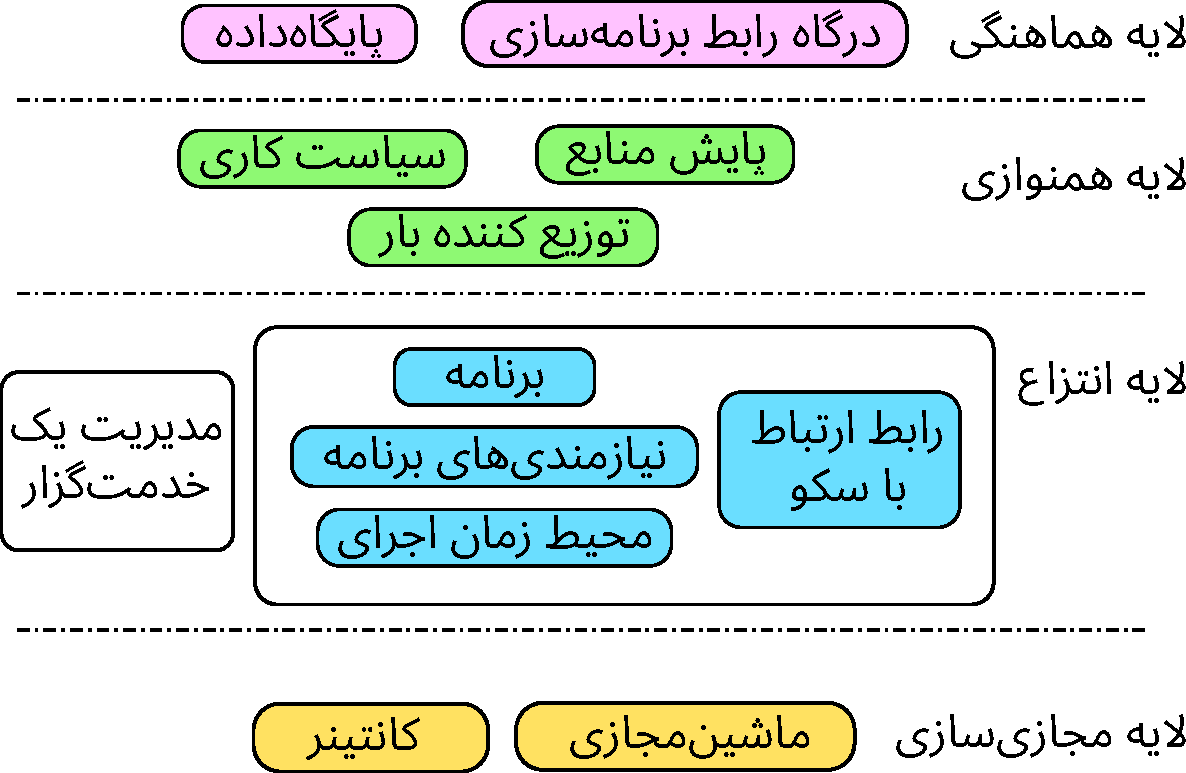
\includegraphics[width=0.5\linewidth]{res/serverless_architecture.pdf}
		\شرح{نگاه سطح بالا به لایه‌های مختلف در سکوهای پردازش بدون‌میزبان}
		\برچسب{معماریسطحبالا}
	\end{figure}
\end{frame}

\begin{frame}{ویژگی‌های برنامه‌های پردازش بدون‌میزبان}
	\begin{itemize}\RTList
	\فقره مولفه‌ها در قالب توابع مبتنی بر رخداد تعریف شده‌اند.
		
	\فقره در هنگام دریافت رخداد یک نسخه از این توابع در یک محیط زمان‌اجرا بارگیری می‌شود و رخداد را پردازش می‌کند.
	
	\فقره در طول اجرا، یک مولفه  می‌تواند دیگر مولفه‌ها را فراخوانی کند و یک زنجیره اجرا ایجاد کند.
		
	\فقره در ذات اجرای مولفه‌ها مواردی همچون \توچشم{همروندی} اجرای چندین مولفه، \توچشم{وقوع اشکال} در زمان اجرا،
		\توچشم{تلاش مجدد یک اجرا} و \توچشم{استفاده مجدد از محیط زمان اجرای} یک مولفه وجود دارد. 
		
	\فقره محیط‌های اجرا در ابتدا سرد هستند و پس از پردازش اطلاعات گرم در نظر گرفته می‌شوند.

	\فقره پس از پایان پردازش یک محیط اجرا می‌تواند بسته شود یا برای مدتی باز بماند.
			\end{itemize}
\end{frame}

%ارائه خدمات بر بستر شبکه اینترنت بخش بزرگی از عرصه پردازش در عصر حاضر را تشکیل داده است و
%فناوری‌های جدیدی مانند اینترنت اشیا و ماشین‌های خودران را امکان پذیر ساخته است. از ملزومات
%ارائه خدمات فراگیر، قابلیت مقیاس پذیری و اتکاپذیری آن است.
%تضمین این دو ویژگی با ایجاد سیستم خدماتی به صورت توزیع شده امکان‌پذیر است. 
%به همین منظور تولید کنندگان سیستم‌های نرم‌افزاری از معماری‌های توزیع شده
%مانند میکروسرویس استفاده می‌کنند.
%
%در این معماری، سیستم به مولفه‌هایی ریزدانه‌ و مستقل تقسیم شده است که با یک دیگر در
%بستر شبکه‌های کامپیوتری در ارتباط هستند. هر مولفه می‌توانند به صورت جداگانه بر روی
%تعدادی خدمت‌رسان اجرا شود. این امر انعطاف لازم را ایجاد می‌کند که در مواقع افزایش
%بار کاری با افزایش تعداد خدمت‌رسان‌ها، مولفه‌ای از سیستم که نیاز به توان بیشتر برای
%پرداز دارد مقیاس پذیرد. همچنین اگر تعدادی از خدمت‌رسان‌ها دچار اشکال شوند، در روند
%کلی خدمت‌رسانی مشکل عمده‌ای رخ نمی‌دهد و تنها شاهد کاهش توان پردازشی خواهیم بود.
%
%در این نوع از سیستم‌ها به دلیل تعدد وجود خدمت‌رسان برای مولفه‌های مختلف نیاز به یک
%توزیع کننده بار کاری میان خدمت‌رسان های موجود است. وظیفه توزیع کننده بار
%است که کل بار موجود را با توجه به سیاست از پیش تعیین شده به نحوی توزیع کند که
%از دید دریافت کننده خدمات تمام خدمت‌رسان‌ها به صورت یک خدمت‌رسان واحد مشاهده شود.
%
%ایجاد و پیاده‌سازی سیستم‌های نرم‌افزاری با ویژگی‌های شرح داده شده هزینه‌بر و دارای
%چالش‌های فنی بسیاری است. از این جهت ارائه دهندگان خدمات زیرساخت و خدمات سکو‌های
%نرم‌افزاری راهکاری با نام پردازش بدون میزبان ارائه کرده‌اند. در این روش، تولید
%کنندگان نرم‌افزار فقط بر روی ایجاد مولفه‌های خود تمرکز می‌کنند و اجزای کاربرد
%خود را با استفاده از چارچوب‌های از پیش تعیین شده پیاده سازی می‌کنند. سپس
%کدهای خود را برای اجرا به ارائه دهنده خدمات پردازش بدون میزبان ارسال می‌کنند.
%
%ارائه دهندگان خدمات پردازش بدون میزبان یک سکوی یک‌پارچه برای اجرای برنامه‌های مشتریان
%خود توسعه داده‌اند که به صورت خودکار برنامه مولفه‌های مختلف را از مشتری دریافت می‌کند و
%آن را بر روی تعدادی خدمت‌گزار اجرا می‌کند.
%وظیفه مقیاس‌پذیری و اتکاپذیری برنامه مشتری بر عهده ارائه دهنده خدمات است و توسط سکوی
%پردازش بدون میزبان به صورت خودکار اجرا می‌شود.
%
%سکو‌های پردازش بدون‌میزبان یک سطح انتزاع برای ایجاد برنامه با قابلیت مقایس‌پذیری بالا
%ارائه کرده اند. در هنگامی که بار میزان بار کاری برنامه تغییر می‌کند، این سکو با توجه
%به نیاز برنامه تعداد خدمت‌رسان‌ها را تنظیم و بار کاری را بین آن‌ها توزیع می‌کند. از این
%منظر توزیع‌بار مناسب میان خدمت‌گزارهای فعال از بخش‌های اساسی این سکوها است.
%
%با توجه به اهمیت سکو‌های پردازش بدون‌میزبان، هدف از این پروژه بررسی و ارزیابی کارایی
%این سکوها با تمرکز ویژه بر روی مولفه توزیع‌بار است. چارچوب‌های پردازش بدون‌میزبان
%باعث بروز برنامه‌هایی شده است که زمان اجرای کوتاهی دارند ولی به صورت متعدد و گسترده
%در مراکز داده اجرا می‌شوند به همین دلیل چالش‌های جدید و متنوعی ایجاد شده است.
%از چند مورد از این چالش‌های می‌توان به 
%سربار قابل توجه محیط زمان اجرا\مرجع{khatri2020potential} و یا کاهش چشمگیر کارایی زمانی
%که برنامه در ابتدای اجرای خود است\مرجع{lloyd2018serverless}.
%تمرکز این پروژه بر روی شناسایی چالش‌ها و بر طرف کردن آن‌ها با توزیع مناسب بار است.
%
%ادامه این بخش به صورتی که در ادامه می‌آید تنظیم شده است. ابتدا به معماری سیستم‌های
%بدون‌میزبان و ساختار اجرای مولفه‌ها پرداخته می‌شود.
%اهمیت سیستم‌های توزیع‌بار شرح داده می‌شود و
%درنهایت روش‌ها ارزیابی کارایی سیستم‌های تحت شبکه درون مراکز داده معرفی می‌گردد.
%
%
%\زیرقسمت{معماری سکو پردازش بدون‌میزبان}
%
%در منابع موجود، پردازش بدون‌میزبان به صورتی که در ادامه می‌آید تعریف شده است.
%این تعریف با روشن ساختن چیستی پردازش بدون‌میزبان به درک بهتر معماری سیستم های
%پردازش بدون‌میزبان کمک می‌کند.
%
%پردازش بدون‌میزبان یک چارچوب پردازش ابری است که یک مدل برنامه سازی سطح بالا
%ارائه می‌کند به نحوی که برنامه ساز می‌تواند برنامه ابری خود را بدون
%نیاز به فعالیت‌های اجرایی مانند تهیه و تخصیص منابع پردازشی ایجاد و اجرا کند.
%وظیفه مسائل مربوط به اتکاپذیری و یا تنظیم توان پردازشی با میزان نیاز برنامه
%بر عهده ارائه دهنده خدمات زیرساخت ابری است. میزان هزینه این خدمات بر اساس
%میزان مصرف واقعی برنامه از منابع موجود محاسبه می‌شود\مرجع{kounev2021toward}.
%
%\begin{figure}[!h]
%	\centering
%	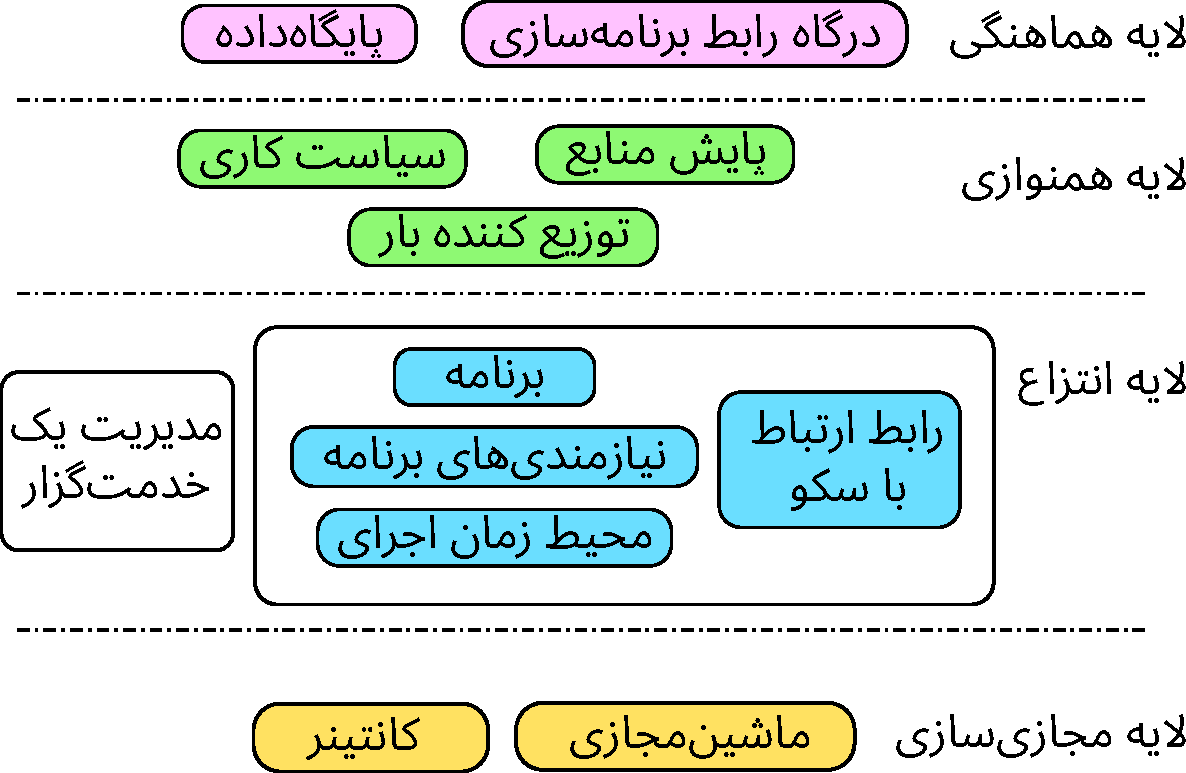
\includegraphics[width=0.5\linewidth]{res/serverless_architecture.pdf}
%	\شرح{نگاه سطح بالا به لایه‌های مختلف در سکوهای پردازش بدون‌میزبان}
%	\برچسب{معماریسطحبالا}
%\end{figure}
%
%همانطور که در شکل \رجوع{معماریسطحبالا} دیده می‌شود، معماری این سیستم‌ها به چهار لایه
%(۱) مجازی‌سازی، (۲) انتزاع، (۳) همنوازی و (۴) هماهنگی ‌تقسیم می‌شود.
%
%لایه مجازیسازی امکان ایزوله کردن برنامه‌های مختلف در حال اجرا بر روی یک سیستم را فراهم می‌کند.
%تکنولوژی‌های پر طرفدار مورد استفاده در این لایه متنوع است ولی استفاده از ماشین‌ مجازی و یا
%کانتینر در این لایه بسیار مرسوم است. لایه مجازیسازی به صورت مجزا بر روی هر خدمت‌گزار اجرا می‌شود.
%
%لایه انتزاع، امکان فراهم سازی محیط اجرای برنامه‌ها و ارتباط میان مولفه‌های مختلف را فراهم می کند.
%در هنگام دریافت یک درخواست از لایه همنوازی، محیط اجرای برنامه که شامل نیازمندی‌ها، سیستم زمان اجرا
%و محیط مجازی است، آماده می‌شود و پردازش در آن صورت می‌گیرد. همچنین اگر نیاز به برقرار ارتباط
%با مولفه‌های دیگر در همین خدمت‌رسان و یا خدمت‌رسان دیگری در مرکز داده باشد، این لایه شیوه‌نامه ارتباطی
%را مشخص می‌کند.
%
%لایه همنوازی وظیفه مقیاس‌پذیری و اتکاپذیری سیستم را دارد. این لایه بار کاری را میان خدمت‌رسان‌ها
%توزیع می‌کند. همچنین موارد مربوط به ردگیری میزان مصرف و پایش سیستم‌ هم در این لایه صورت می‌گیرد.
%
%لایه هماهنگی مواردی همچون درگاه رابط برنامه‌نویسی، پایگاه‌های داده، زیر سیستم‌های مربوط به کارهای
%توسعه و عملیات اجرایی را در بر می‌گیرد.
%
%\زیرقسمت{ساختار مولفه‌ها در پردازش بدون‌میزبان}
%\برچسب{ساختارمولفه}
%
%\begin{figure}[!h]
%	\centering
%	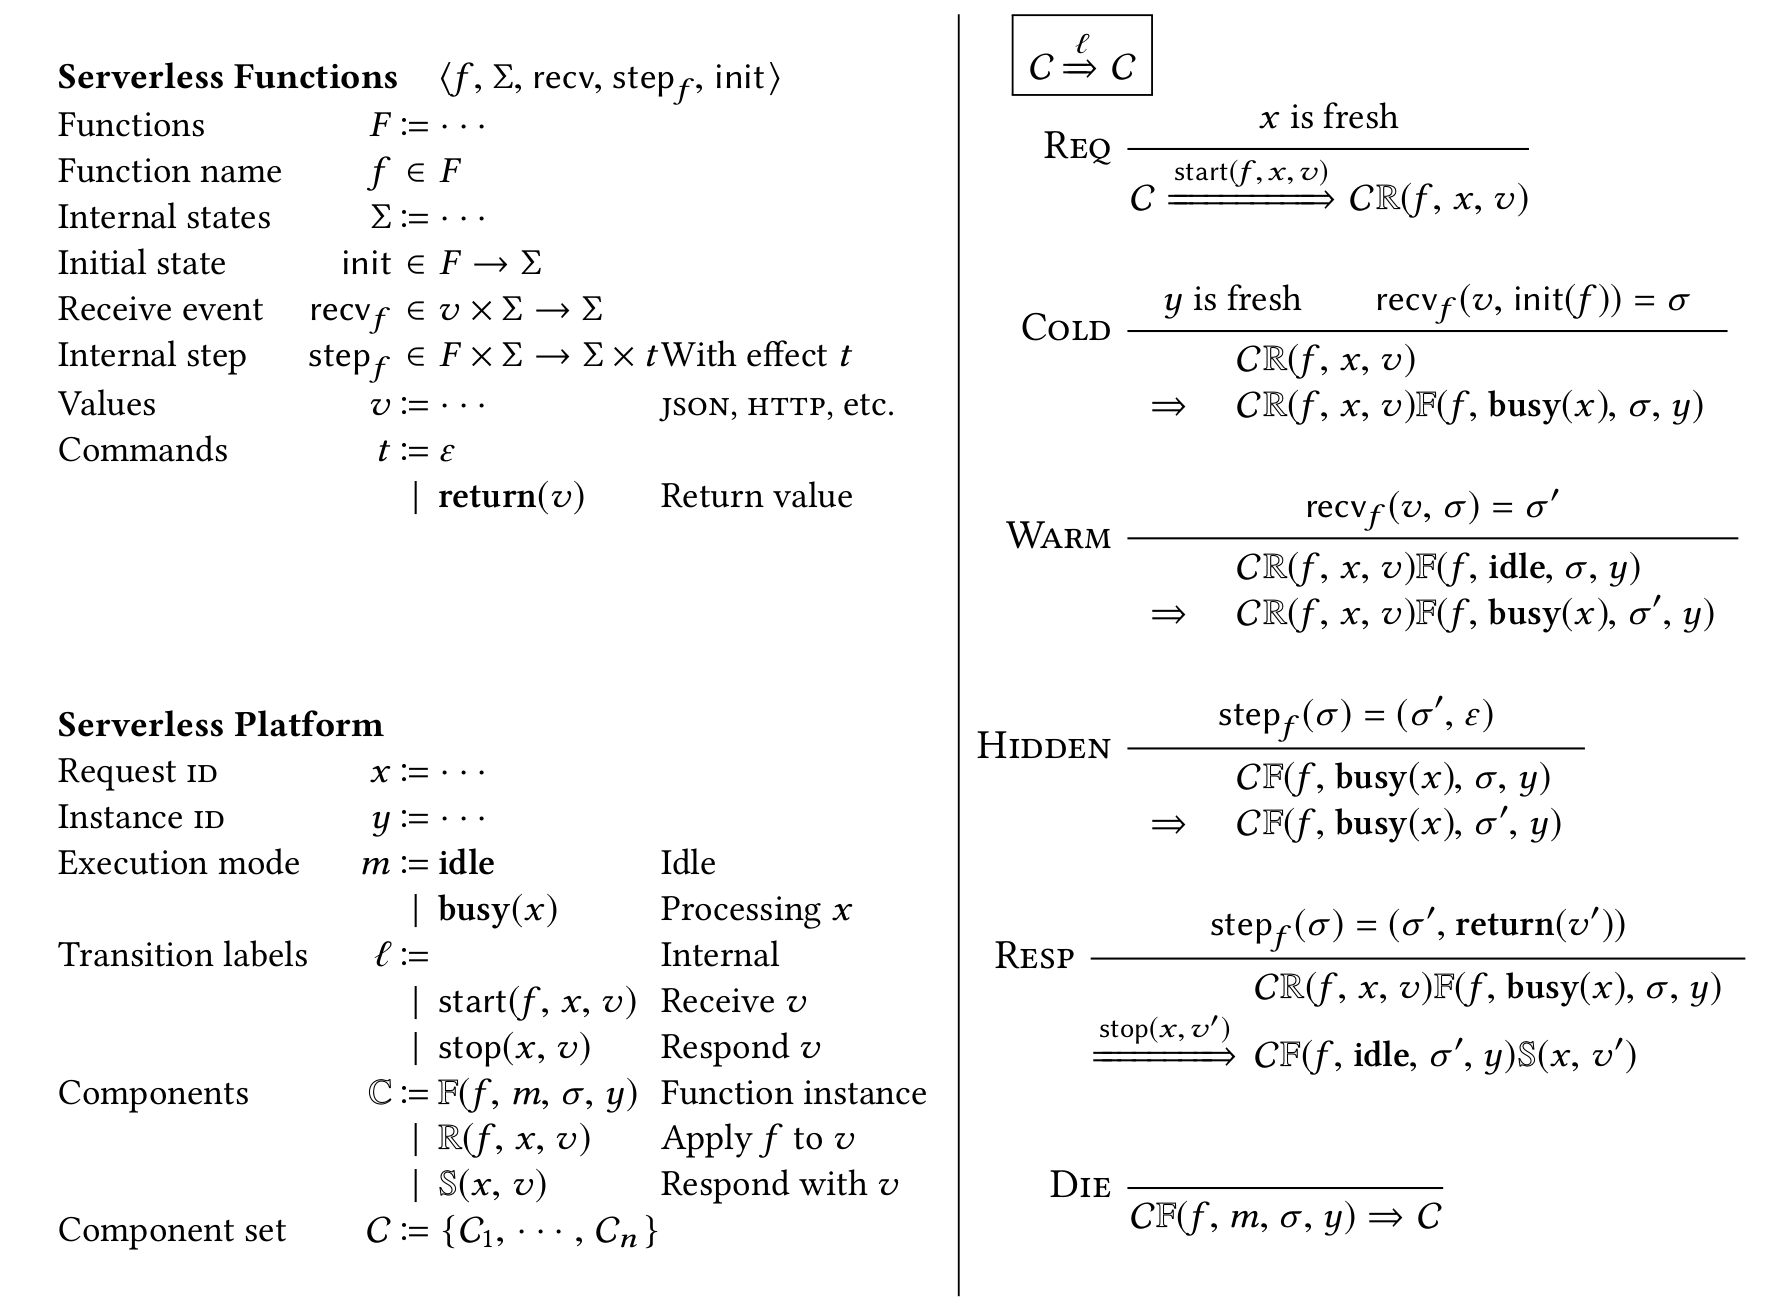
\includegraphics[width=0.9\linewidth]{res/sos.png}
%	\شرح{مدل معناشناسی ساخت‌یافته عملیاتی برای مولفه‌های پردازش بدون‌میزبان (برگرفته از \مرجع{jangda2019formal})}
%	\برچسب{سوس}
%\end{figure}
%
%ایجاد کنندگان نرم‌افزار مولفه‌های خود را در قالب توابعی که به صورت مبتنی بر رخداد تعریف شده‌اند،
%تشکیل می‌دهند. در هنگام دریافت رخدادهای مورد نظر یک مولفه، یک نسخه از این توابع در یک محیط زمان اجرا
%بارگیری می‌شود و رخداد را پردازش می‌کند. در طول اجرا، یک مولفه  می‌تواند دیگر مولفه‌ها را فراخوانی کند
%و در نتیجه یک زنجیره اجرا از مولفه‌ها را تشکیل دهد.
%
%در ذات اجرای مولفه‌ها مواردی همچون همروندی اجرای چندین مولفه، وقوع اشکال در زمان اجرا،
%تلاش مجدد یک اجرا و استفاده مجدد از محیط زمان اجرای یک مولفه وجود دارد. تمام این موارد
%باعث پیچیدگی مفهومی توابع مورد نظر می‌شود. برای درک بهتر از ساختار برنامه سازی سیستم‌های
%بدون‌میزبان مدل معناشناسی ساخت‌یافته عملیاتی در شکل \رجوع{سوس} ارائه شده است\مرجع{jangda2019formal}.
%
%برای هر مولفه $f$ می‌تواند در هر زمان یک درخواست بیاید که به آن یک شناسه منحصر به فرد $x$ نسبت داده شده‌است
%(قاعده $Req$).
%در خواست دریافت شده یا منجر به ایجاد یک محیط اجرا جدید می‌شود (قاعده $Cold$) و یا در یک محیط اجرای از پیش
%آمده ادامه پردازش می‌شود (قاعده $Warm$). مراحل اجرای پردازش از دید این مدل پنهان است (قاعده $Hidden$).
%در نهایت پس از ایجاد پاسخ پردازش (قاعده $Resp$) محیط پردازش آزاد می‌شود و می‌تواند دوباره مورد استفاده قرار 
%بگیرد و یا اینکه محیط اجرا بسته می‌شود (قاعده $Die$).
%
%
%\زیرقسمت{چالش‌های توزیع‌بار در سکو‌های پرداز بدون‌میزبان}
%
%توزیع‌بار کاری میان خدمت‌گزاران مختلف از این جهت حائز اهمیت است که زمان‌بندی اجرای برنامه‌ها،
%تعداد خدمت‌گزاران فعال برای پردازش و اعمال سیاست‌های تضمین کیفیت خدمات از جمله وظایف آن است.
%
%برنامه‌‌هایی که در سکو پردازش بدون‌میزبان اجرا می‌شوند نیازهای متنوعی دارند. یک مطالعه نشان می‌دهد
%که اندازه برنامه‌ها از یک مولفه تا صدها مولفه متغییر است و زمان اجرای هر کدام از مولفه در بازه‌ی
%کمتر از یک ثاینه تا چندین دقیقه تغییر می‌کند \مرجع{tariq2020sequoia}.
%
%در هنگام دریافت یک رخداد، توزیع کننده بار باید ابتدا با توجه نوع رخداد فرآیند زمانبندی را انجام
%دهد و سپس با توجه به حالت خدمت‌گزارهای مرکز داده، درخواست را به یک خدمت‌گزار تحویل دهد. دو مسئله
%در این موضوع وجود دارد. اول اینکه هر کدام رخداد در چه زمانی به خدمت‌گزار ارسال شود. دوم آنکه
%درخواست به کدام خدمت‌گزار ارسال شود.
%
%زمان ارسال درخواست به خدمت‌گزار، برای تضمین کیف خدمات بسیار اثر گذار است. از طرفی عملیات
%زمانبندی نیاز به حافظه برای میانگیری درخواست‌های در حال انتظار دارد. اگر حافظه تخصیص داده
%شده پر شود آنگاه درخواست‌های  مازاد ارسال شده طرد می‌شوند.
%
%انتخاب خدمت‌گزاری که قرار است درخواست را پردازش کند نیز از اهمیت بالایی برخوردار است. اگر
%نیاز باشد که یک محیط اجرای جدید روی خدمت‌گزار ایجاد شود، این عملیات زمانبر خواهد بود.
%همچنین کارایی‌ محیط اجرایی که به تازگی ایجاد شده است (در حالت سرد است) از اجرای درخواست در یک
%محیط که از قبل وجود داشته شده است (در حالت گرم است) می‌تواند تا ۱۵ برابر کندتر باشد\مرجع{lloyd2018serverless}.
%
%
%\زیرقسمت{ارزیابی کارایی مراکز داده}
%
%برای ارزیابی کارایی سیستم‌های مراکز داده روش های گوناگونی وجود دارد. در این پروژه بر روی
%تئوری صف تمرکز شده است.
%
%\زیرزیرقسمت{تئوری صف}
%
%\begin{figure}[!h]
%	\centering
%	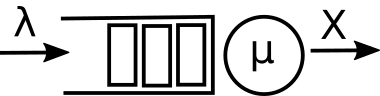
\includegraphics[width=0.3\linewidth]{res/queue.png}
%	\شرح{نمایش یک صف در مدل تئوری صف}
%	\برچسب{صف}
%\end{figure}
%
%در تئوری صف یک واحد پردازش به صورتی که در شکل \رجوع{صف} مشاهده می‌شود نمایش داده می‌شود.
%در این مدل با دانستن توزیع احتمالاتی رخداد‌ها و نرخ ورود و نرخ پردازش با استفاده از روش‌های تحلیلی مواردی از جمله 
%زمان انتظار و گذردهی سیستم محاسبه می‌شود. از چالش‌های استفاده این مدل برای سکوهای پردازش بدون‌میزبان تغییر
%تعداد خدمت‌گزاران، نرخ ورود و نرخ خروج سیستم به صورت پیوسته است. با ایجاد یک محیط اجرای جدید در واقع یک 
%صف جدید به مدل اضافه شده است و چون محیط اجرا در ابتدا در حالت سرد قرار دارد پس نرخ سرویس‌ دهی پایینی دارد
%با گرم شدن محیط اجرا، نرخ سرویس دهی افزایش پیدا می‌کند. در هنگامی که یک محیط اجرا بسته می‌شود یک صف از مدل
%حذف می‌شود. این تغییرات محاسبات تحلیلی را با چالش‌های فراوان همراه می‌سازد.
%
%یک روش دیگر برای محاسبه کارایی این سیستم‌ها استفاده از شبیه‌سازی است. با ایجاد مدل تئوری صف می‌توان محیط‌های شبیه‌سازی
%را با پارامترهای معین ایجاد کرد و با اجرای شبیه‌سازی برای تعداد زیادی از درخواست‌ها و به صورت مکرر می‌توان کارایی
%سیستم را ارزیابی کرد.
%% Related works
\section{کارهای مرتبط پیشین}

\begin{frame}{توزیع‌بار کاری در سکو‌های پرداز بدون‌میزبان}
\begin{itemize}\RTList
	\فقره سرعت ایجاد محیط اجرا یک چالش‌ برای کارایی سکو پردازش بدون‌میزبان است.
	
	\فقره 	برای ایجاد محیط اجرا باید نیازمندی‌ها بار گیری و اجرا شوند.
%	(کتابخانه‌ها، برنامه‌های شخص ثالث و سیستم زمان اجرا)
	
	\فقره به همین منظور خدمت‌گزاران این نیازمندی‌ها را در یک حافظه نهان نگهداری می‌کنند.
\end{itemize}
	
\centering{
\mybox{کار مرتبط}{
	\مل{PASch} یک سیستم توزیع‌بار است که با توجه به نیازمندی‌های بارگیری شده روی خدمت‌گزارها
	گذردهی سیستم‌ را $1.29$ برابر افزایش  و تاخیر صدک ۸۰ام را تا ۲۳ برابر
	کاهش داده است\مرجع{aumala2019beyond}.
}}
\end{frame}


\begin{frame}{توزیع‌بار کاری در سکو‌های پرداز بدون‌میزبان}
	\begin{itemize}\RTList
		\فقره محیط‌های اجرا در حالت سرد عملکرد ضعیف‌تری نسبت به محیط گرم دارند.
		
		\فقره محیط‌های اجرا پس از اتمام کار برای مدتی باز نگه‌داشته می‌شوند.
		
		\فقره توزیع‌کننده بار می‌تواند با آگاهی از محیط‌های گرم کارایی را بهبود دهد.
	\end{itemize}
	
	\centering{
		\mybox{کار مرتبط}{
			با افزودن آگاهی از مکان محیط‌های گرم به توزیع‌کننده بار،
			نشان داده شده است که می‌توان ۶۳ درصد تاخیر در صدک ۹۹‌ام را کاهش داد\مرجع{wu2022container}.
	}}
\end{frame}


\begin{frame}{توزیع‌بار کاری در سکو‌های پرداز بدون‌میزبان}
	\begin{itemize}\RTList
		\فقره تشخیص زمان بستن یک محیط اجرا اهمیت فراوانی دارد.
		
		\فقره اگر محیط اجرا فورا بسته شود تعداد محیط‌های سرد ایجاد شده افزایش پیدا می‌کند.
		
		\فقره اگر محیط اجرا بسته نوشد هزینه خدمات بسیار زیاد می‌شود.
		
		\فقره تمام مولفه‌ها فرکانس فراخوانی یکسانی ندارند.
	\end{itemize}
	
	\centering{
		\mybox{کار مرتبط}{
			با پایش و جمع‌آوری آمار فراخوانی مولفه‌های مختلف روش‌هایی برای تعیین مدت زمان
			مناسب برای باز نگهداشتن یک محیط اجرا پیشنهاد شده است \مرجع{shahrad2020serverless}.
	}}
\end{frame}

\begin{frame}{توزیع‌بار کاری در سکو‌های پرداز بدون‌میزبان}
	
	\centering{
		\mybox{کار مرتبط}{
			برای اجرای کاربرد‌های
			بلادرنگ نیاز است تا تضمین پایان پردازش تا موعد مقرر رخداد ارائه شود.
			به همین منظور پیاده‌سازی یک الگوریتم آگاه از موعد رخدادها و توان پردازشی موجود
			نیاز است\مرجع{mampage2021deadline}.	}}
	\centering{
	\mybox{کار مرتبط}{
		تضمین کیفیت سرویس برای ارائه دهندگان خدمات ابری اهمیت دارد.
		از این منظر پیاده سازی الگوریتم‌های مختلف که
		انصاف را برای انواع بارهای کاری رعایت کند اهمیت دارد\مرجع{tariq2020sequoia}.}}

	\centering{
	\mybox{کار مرتبط}{
		ارسال پیام از یک خدمت‌گزار به یک خدمت‌گزار دیگر زمان‌بر است. از این روی طراحی سیستم
		توزیع‌بار به نحوی که زنجیره اجرا بر روی یک خدمت‌گزار قرار بگیرد باعث
		افزایش کارایی می‌شود\مرجع{jia2021nightcore}.
	}}

\end{frame}


\begin{frame}
	\begin{table}[!h]
		\centering
		\شرح{جمع‌بندی کارهای مرتبط}
		\برچسب{کارهایپیشین}
		\begin{tabular}{|c|c|c|r|}
			\hline
			مرجع & سال انتشار & استفاده از مدل تحلیلی & \multicolumn{1}{c|}{معیار مورد توجه}   \\ \hline
			\مرجع{mahmoudi2020performance}    & ۲۰۱۹       & بله                   & ارزیابی کارایی                         \\ \hline
			\مرجع{lin2020modeling}    & ۲۰۲۰       & بله                   & هزینه سرویس در مقابل کارایی            \\ \hline
			\مرجع{mampage2021deadline}   & ۲۰۲۱       & خیر                   & توجه به نیاز سیستم‌های بی درنگ         \\ \hline
			\مرجع{lee2021greedy}       & ۲۰۲۱       & خیر                   & افزایش بهره‌وری حافظه نهان             \\ \hline
			\مرجع{shahrad2020serverless}          & ۲۰۲۰       & خیر                   & تعداد محیط های اجرای سرد               \\ \hline
			\مرجع{aumala2019beyond}    & ۲۰۱۸       & خیر                   & توجه به حافظه نهان نیازمندی‌های برنامه \\ \hline
			\مرجع{wu2022container}   & ۲۰۲۲       & خیر                   & توجه به چرخه‌حیات لایه مجازی‌سازی      \\ \hline
			\مرجع{jia2021nightcore}   & ۲۰۲۱       & خیر                   & توجه به اجرای زنجیره روی یک خدمت‌گزار      \\ \hline
		\end{tabular}
	\end{table}
\end{frame}

%
%پردازش بدون‌میزبان عرصه جدیدی در پردازش ابری است که توجه پژوهشگران بسیاری
%را به خود جلب کرده است. در این بخش کارهای مرتبط را در زمینه‌های توزیع‌بار،
%ارزیابی کارایی و مدل‌سازی سکو‌های پردازش بدون‌میزبان بررسی می‌‌شود.
%
%
%\زیرقسمت{توزیع‌بار کاری در سکو‌های پرداز بدون‌میزبان}
%
%سرعت ایجاد محیط اجرا یکی از چالش‌های کارایی سیستم‌های پردازش بدون‌میزبان. برای
%ایجاد محیط اجرا با نیازمندی‌ها که شامل کتابخانه‌ها، برنامه‌های شخص ثالث و سیستم زمان اجرا
%است بار گیری و اجرا شوند. به همین منظور خدمت‌گزاران این نیازمندی‌ها را برای مولفه‌هایی که
%به تازگی اجرا کرده‌اند در یک حافظه نهان نگهداری می‌کنند تا در صورت نیاز به اجرای مجدد کارایی
%بهتری را ارائه کنند. \مل{PASch} یک سیستم توزیع‌بار است که با توجه به این موضوع توانسته است
%گذردهی این سیستم‌ها را $1.29$ برابر افزایش دهد و تاخیر صدک ۸۰ام را تا ۲۳ برابر
%کاهش دهد\مرجع{aumala2019beyond}.
%
%یکی دیگر از چالش‌هایی کارایی سیستم‌های پردازش بدون‌میزبان، عملکرد ضعیف محیط اجرا در حالت سرد است.
%به همین منظور ارائه دهندگان این خدمات، پس از پایان کار یک مولفه، محیط اجرای آن را برای مدتی فعال
%نگاه می‌دارند تا بتوان از آن استفاده مجدد کرد. متاسفانه سیستم توزیع کننده بار کاری از محیط‌های اجرای
%گرم آگاه نیست و به همین منظور نمی‌تواند از این قابلیت بهره کافی را ببرد. با افزودن این آگاهی در
%هنگام توزیع‌بار نشان داده شده است که می‌توان ۶۳ درصد تاخیر در صدک ۹۹‌ام را کاهش داد\مرجع{wu2022container}.
%
%کاربردهای بلادرنگ در دنیای پردازش از جایگاه خاصی برخوردار هستند.برای اجرای برنامه‌های
%بلادرنگ در سکو‌های پردازش بدون‌میزبان نیاز است تا تضمین پایان پردازش تا موعد مقرر رخداد
%ارائه شود. به همین منظور پیاده‌سازی یک الگوریتم آگاه از موعد رخدادها و توان پردازشی موجود
%نیاز است\مرجع{mampage2021deadline}.
%
%تضمین کیفیت سرویس برای ارائه دهندگان خدمات ابری بسیار حیاتی است. سیستم‌های توزیع‌بار 
%بهترین مکان برای اعمال سیاست‌های مختلف است. از این منظر پیاده سازی الگوریتم‌های مختلف که
%انصاف را برای انواع بارهای کاری رعایت کند اهمیت دارد\مرجع{tariq2020sequoia}.
%
%ارسال پیام از یک خدمت‌گزار به یک خدمت‌گزار دیگر زمان‌بر است. از این روی طراحی سیستم
%توزیع‌بار به نحوی که زنجیره اجرا تا جای ممکن بر روی یک خدمت‌گزار قرار بگیرد باعث
%افزایش کارایی می‌شود\مرجع{jia2021nightcore}.
%
%
%\زیرقسمت{ارزیابی کارایی سکو‌های پردازش بدون‌میزبان}
%
%ارزیابی کارایی سکو‌های پردازش بدون‌میزبان مورد توجه بسیاری قرار گرفته است.
%این مطالعات باعث می‌شود گلوگاه‌ها و نقاط ضعف سیستم‌ها مشخص شود و در نتیچه
%بتوان با طراحی بهتر سیستم‌ها کارایی بالاتری را دریافت کرد\مرجع{palade2019evaluation}.
%
%دو راهبرد برای ارزیابی کارایی سیستم‌های پردازش ابری مورد استفاده است. در روش اول 
%مطالعات مشاهداتی صورت می‌گیرد به این طریق که با اجرای بارهای کاری بر روی سیستم‌ها و
%جمع‌آوری مشاهدات و نتایج، درنهایت مقایسه‌ای میان روش‌های مختلف صورت می‌گیرد.
%در این روش بدست آوردن اطلاعات دقیق و قابل تکرار از چالش‌های موجود است. روش دیگر
%استفاده از مدل‌های تحلیلی است. طراحی این مدل‌ها دشوار است و ممکن است جزئیات مهمی
%را در هنگام ایجاد لایه‌های انتزاع از درست بدهند\مرجع{kounev2021toward}.
%
%در ارزیابی سیستم‌های بدون‌میزبان پارامتر‌های متعددی مورد توجه است که از جمله‌ی
%آن‌ها می‌توان به زمان اجرا، گذردهی، تعداد دفعات فراخوانی یک مولفه و زمان ایجاد محیط اجرا
%اشاره کرد\مرجع{shahrad2020serverless,ustiugov2021analyzing}.
%
%
%\زیرقسمت{مدل‌سازی سکو‌های پردازش بدون‌میزبان}
%
%با توجه به ذات توزیع شده سیستم‌های بدون‌میزبان و انجام آزمایش‌های
%مشاهداتی با چالش‌های بسیاری مواجه است.
%از جمله چالش تفاوت چشمگیر در روش‌های پیاده سازی سکو‌های پردازش بدون‌میزبان
%توسط ارائه دهندگان مختلف است. از این جهت مطالعات صورت گرفته برای قابل
%قیاس بودن باید بر روی چندین سکوی مختلف به صورت متناسب صورت
%بگیرد\مرجع{palade2019evaluation, mcgrath2017serverless}.
%از طرف دیگر، بارهای کاری پردازش بدون‌میزبان متفاوت است و مطالعات مشاهداتی
%فقط برای یک حوزه می‌تواند کاربردی باشد.
%در صورت انجام چنین مشاهداتی، اطلاعات بدست آمده در کاربرد مورد مطالعه بسیار
%ارزشمند است\مرجع{shahrad2020serverless}.
%
%
%با توجه به پیچیدگی‌های انجام آزمایش‌های مشاهداتی، انجام شبیه‌سازی‌ جنبه‌های
%مختلف سکوی ارائه خدمات بسیار مورد توجه قرار گرفته شده
%است\مرجع{shahrad2020serverless,mahmoudi2021simfaas,jeon2019cloudsim}.
%معمولا شبیه‌سازی‌ها بر روی ویژگی‌های محدودی از معیارهای کارایی تمرکز می کنند.
%مواردی مانند تعداد محیط‌های سرد ایجاد شده یا تعداد پیام‌های از دست رفته از جمله
%این معیارها است.
%
%استفاده از روش‌های تحلیلی باعث فهم ویژگی‌های ذاتی موضوع مورد مطالعه می‌شوند. این
%روش‌ها امکان مقایسه پیاده‌سازی‌های عملی را با حدبالای تئوری قابل دست‌یابی می‌دهند و به
%طراحان کمک می‌کنند که درباره جنبه‌های مختلف سیستم تصمیم بگیرند.
%از طرفی بدست‌آوردن مدل‌های تحلیلی همیشه ممکن نیست.
%در کار‌های گذشته تلاش‌هایی برای مدل‌سازی سکو‌های پردازش بدون‌میزبان ارائه 
%شده است\مرجع{mahmoudi2020performance,lin2020modeling,mampage2021deadline,lee2021greedy}.
%مدل‌های بدست آمده امکان بهینه‌سازی چندین ويزگی حائز اهمیت مانند، کارایی و هزینه
%مورد نیاز سیستم را فراهم می‌آورد.
%
%در جدول \رجوع{کارهایپیشین} خلاصه‌ای از رویکرد کارهای پیشین به بررسی این مسئله پرداخته شده است.
%
%\begin{table}[!h]
%	\centering
%	\شرح{جمع‌بندی کارهای مرتبط}
%	\برچسب{کارهایپیشین}
%	\begin{tabular}{|c|c|c|r|}
%		\hline
%		مرجع & سال انتشار & استفاده از مدل تحلیلی & \multicolumn{1}{c|}{معیار مورد توجه}   \\ \hline
%		\مرجع{mahmoudi2020performance}    & ۲۰۱۹       & بله                   & ارزیابی کارایی                         \\ \hline
%		\مرجع{lin2020modeling}    & ۲۰۲۰       & بله                   & هزینه سرویس در مقابل کارایی            \\ \hline
%		\مرجع{mampage2021deadline}   & ۲۰۲۱       & خیر                   & توجه به نیاز سیستم‌های بی درنگ         \\ \hline
%		\مرجع{lee2021greedy}       & ۲۰۲۱       & خیر                   & افزایش بهره‌وری حافظه نهان             \\ \hline
%		\مرجع{shahrad2020serverless}          & ۲۰۲۰       & خیر                   & تعداد محیط های اجرای سرد               \\ \hline
%		\مرجع{aumala2019beyond}    & ۲۰۱۸       & خیر                   & توجه به حافظه نهان نیازمندی‌های برنامه \\ \hline
%		\مرجع{wu2022container}   & ۲۰۲۲       & خیر                   & توجه به چرخه‌حیات لایه مجازی‌سازی      \\ \hline
%		\مرجع{jia2021nightcore}   & ۲۰۲۱       & خیر                   & توجه به اجرای زنجیره روی یک خدمت‌گزار      \\ \hline
%	\end{tabular}
%\end{table}


%% Solution
\documentclass[12pt]{article}
\usepackage[margin=1in,footskip=0.25in]{geometry}
\usepackage{titlesec}
\usepackage{graphicx}
\usepackage{amsmath}

% Import listings for code representation
\usepackage{listings}
\usepackage{color}
\usepackage{xcolor}

\definecolor{mygreen}{rgb}{0,0.6,0}
\definecolor{mygray}{rgb}{0.5,0.5,0.5}
\definecolor{mymauve}{rgb}{0.58,0,0.82}
\lstset
  {backgroundcolor=\color{white},  % choose the background color; you must add \usepackage{color} or \usepackage{xcolor}; should come as last argument
  basicstyle=\footnotesize\ttfamily,        % the size of the fonts that are used for the code
  breakatwhitespace=false,         % sets if automatic breaks should only happen at whitespace
  breaklines=true,                 % sets automatic line breaking
  captionpos=b,                    % sets the caption-position to bottom
  commentstyle=\color{mygreen},    % comment style
  deletekeywords={},               % if you want to delete keywords from the given language
  escapeinside={\%*}{*)},          % if you want to add LaTeX within your code
  extendedchars=true,              % lets you use non-ASCII characters; for 8-bits encodings only, does not work with UTF-8
  firstnumber=1,                   % start line enumeration with line 1000
  frame=single,                    % adds a frame around the code
  keepspaces=true,                 % keeps spaces in text, useful for keeping indentation of code (possibly needs columns=flexible)
  keywordstyle=\color{blue},       % keyword style
  language=c++,                    % the language of the code
  morekeywords={},                 % if you want to add more keywords to the set
  numbers=left,                    % where to put the line-numbers; possible values are (none, left, right)
  numbersep=5pt,                   % how far the line-numbers are from the code
  numberstyle=\tiny\color{mygray}, % the style that is used for the line-numbers
  rulecolor=\color{black},         % if not set, the frame-color may be changed on line-breaks within not-black text (e.g. comments (green here))
  showspaces=false,                % show spaces everywhere adding particular underscores; it overrides 'showstringspaces'
  showstringspaces=false,          % underline spaces within strings only
  showtabs=false,                  % show tabs within strings adding particular underscores
  stepnumber=2,                    % the step between two line-numbers. If it's 1, each line will be numbered
  stringstyle=\color{mymauve},     % string literal style
  tabsize=2,                       % sets default tabsize to 2 spaces
  title=\lstname,                  % show the filename of files included with \lstinputlisting; also try caption instead of title
}

% Import these packages for drawing markov chains
\usepackage{tikz}
\usetikzlibrary{automata, positioning}

\usepackage{fancyhdr}

% xepersian should be the last package that is loaded
\usepackage[localise=on]{xepersian}
\settextfont{XB Niloofar}
% \settextfont{BNazanin}
\setlatintextfont{Crimson}
% ------------------------------------------------------------------------------

\titleformat{\section}
  {\normalfont\Large\bfseries}   % The style of the section title
  {}                             % a prefix
  {0pt}        % How much space exists between the prefix and the title
  {\quad}    % How the section is represented

% Title Definition
\def \mytitletext {نام درس مربوطه}
\def \myauthorname {نام و نام خانوادگی}
\def \mysubtitle{اسم این سری از تمرین}
\def \mystdno{(شماره دانشجویی)}
\def \myuniversity{نام دانشگاه}
\def \mydepartment{نام دانشکده}
\def \mylogo{res/logo.pdf}  % نشان دانشگاه

% ------------------------------------------------------------------------------
\newcommand{\mytitle}{
  % Logo
  \begin{tabular}{cc}
    \includegraphics[width=0.1\linewidth]{\mylogo} &
    \raisebox{0.05\linewidth}
    {\begin{tabular}{c}
      \myuniversity \\
      \mydepartment
    \end{tabular}}
  \end{tabular}
  % Title
  \begin{center}
  {\Huge\textbf{\mytitletext}\par}
  \vspace{3mm}
  {\Large\textbf\mysubtitle\par}
  \vspace{5mm}
  {\large\myauthorname \\ \mystdno \par}
  \end{center}
}

\pagestyle{fancy}
\chead{\mytitletext}
\lhead{\myauthorname}

% Command Definitions
\newcommand{\myhline}{\noindent\rule[0.5ex]{\linewidth}{1pt}\par}
\newcommand{\زیرل}[1]{\footnote{\lr{#1}}}
\def\مل{\lr}
% ------------------------------------------------------------------------------

% Document Specific Definitions
% ------------------------------------------------------------------------------


\begin{document}
\mytitle

% Problem one
\section{سوال یک}
این یک متن تستی است و هیچ معنای خاصی ندارد. شرط زیر را می‌توان دید.
($\lambda < \mu $).
برای پاسخ به این سوال معادلات را می‌نویسیم.

\begin{align}
t_1 + X_3 = X_1 \\
X_1 . P_{13} + X_2 . P_{23} + t_3 = X_2 \\
X_1 . P_{12} + t2 = X_2
\end{align}

از روابط بالا می‌توان نتیجه گرفت که :

\begin{equation}
X_1 . P_{13} + [ X_1 . P_{12} + r2 ] . P_{23} + r_3 = X_1 - r_1
\end{equation}


متن تستی در ادامه دیده می‌شود این متن هیچ پاسخ به خصوصی را همراه ندارد.
تلاش شده است تا جوابی که این پاسخ آن بوده است حذف شود.

\begin{equation}
X_{{max}} = {1 \over 5} t^2 + 3t + 7 = 10    
\end{equation}

در نتیجه بیشینه مقدار ممکن برای
$r_1$
عبارت است از:

\begin{equation}
    y = x^2 + 56z + \int_a^b f(x) \mathrm{d}x
\end{equation}

\pagebreak

% Problem two
\section{سوال دوم}
\subsection{الف}


\[
\begin{tikzpicture}
    \node[state](p0){آفتابی};
    \node[state, right=of p0](p1){ابری};
    \node[state, right=of p1](p2){بارانی};
    \draw[every loop]
    (p0) edge[bend right, auto=right] node{$0.5$} (p1)
    (p0) edge[loop above] node{$0.5$} (p1)
    (p1) edge[bend right, auto=right] node{$0.4$} (p0)
    (p1) edge[bend right, auto=right] node{$0.2$} (p2)
    (p1) edge[loop above] node{$0.4$} (p1)
    (p2) edge[bend right, auto=right] node{$0.5$} (p1)
    (p2) edge[loop above] node{$0.5$} (p2);
\end{tikzpicture}
\]

\begin{equation}
    P = 
    \begin{bmatrix}
        0.5 & 0.5 & 0  \\
        0.4 & 0.4 & 0.2 \\
        0  & 0.5 & 0.5
    \end{bmatrix}
\end{equation}


\subsection{ب}

\textbf{یک ویژگی}\\

متن تستی که اینجا آمده است فقط برای پر کردن فضای متن قبلی است و هیچ منظور خاصی از نوشتن آن وجود ندارد.
متن تستی که اینجا آمده است فقط برای پر کردن فضای متن قبلی است و هیچ منظور خاصی از نوشتن آن وجود ندارد.
\\

\noindent \textbf{ویژگی دیگر}\\

متن تستی که اینجا آمده است فقط برای پر کردن فضای متن قبلی است و هیچ منظور خاصی از نوشتن آن وجود ندارد.
متن تستی که اینجا آمده است فقط برای پر کردن فضای متن قبلی است و هیچ منظور خاصی از نوشتن آن وجود ندارد.
متن تستی که اینجا آمده است فقط برای پر کردن فضای متن قبلی است و هیچ منظور خاصی از نوشتن آن وجود ندارد.
\\

\noindent \textbf{ویژگی دیگر دوم}\\

متن تستی که اینجا آمده است فقط برای پر کردن فضای متن قبلی است و هیچ منظور خاصی از نوشتن آن وجود ندارد.
متن تستی که اینجا آمده است فقط برای پر کردن فضای متن قبلی است و هیچ منظور خاصی از نوشتن آن وجود ندارد.
متن تستی که اینجا آمده است فقط برای پر کردن فضای متن قبلی است و هیچ منظور خاصی از نوشتن آن وجود ندارد.

\pagebreak
\subsection{ج}
متن تستی که اینجا آمده است فقط برای پر کردن فضای متن قبلی است و هیچ منظور خاصی از نوشتن آن وجود ندارد.
متن تستی که اینجا آمده است فقط برای پر کردن فضای متن قبلی است و هیچ منظور خاصی از نوشتن آن وجود ندارد.
متن تستی که اینجا آمده است فقط برای پر کردن فضای متن قبلی است و هیچ منظور خاصی از نوشتن آن وجود ندارد.

\begin{align}
    \vec{\pi} . P = \vec{\pi} \\
    \sum_{0}^{2} \! \pi_i \, = \pi_0 + \pi_1 + \pi_2 =  1
\end{align}

با جاگذاری ماتریس
$ P $
و بردار
$\vec{\pi} = < \pi_0, \pi_1, \pi_2 >$
در رابطه بالا و حل معادلات خواهیم داشت:

\begin{align}
    0.5 \rho_0 + 0.7 z_1 = X_0 \Rightarrow \rho_0 = 0.8 \pi_1 \\
    \pi_1 = \frac{52}{101} \\
    \pi_0 = \frac{34}{111} \\
    \pi_2 = \frac{21}{111}
\end{align}

حال با داشتن بردار 
$\vec{\pi}$
متن تستی که اینجا آمده است فقط برای پر کردن فضای متن قبلی است و هیچ منظور خاصی از نوشتن آن وجود ندارد.

\vspace{0.5cm}
\noindent
\textbf{(۱) یک بخش از سوال.}

متن تستی که اینجا آمده است فقط برای پر کردن فضای متن قبلی است و هیچ منظور خاصی از نوشتن آن وجود ندارد.
متن تستی که اینجا آمده است فقط برای پر کردن فضای متن قبلی است و هیچ منظور خاصی از نوشتن آن وجود ندارد.
متن تستی که اینجا آمده است فقط برای پر کردن فضای متن قبلی است و هیچ منظور خاصی از نوشتن آن وجود ندارد.
متن تستی که اینجا آمده است فقط برای پر کردن فضای متن قبلی است و هیچ منظور خاصی از نوشتن آن وجود ندارد.

\begin{align}
    P(\text{حالت اول} | \text{حالت دوم}) =
        {P(\text{حالت اول} \cap \text{حالت دوم}) \over P( \text{حالت دوم}) } \\
    P(\text{حالت اول} | \text{حالت دوم }) = {\frac{45}{114} \over \frac{37}{121}} = \frac{57}{67}
\end{align}


\pagebreak
\noindent
\textbf{(۲) در دو روز گذشته چتر همراهش بوده باشد.}

متن تستی که اینجا آمده است فقط برای پر کردن فضای متن قبلی است و هیچ منظور خاصی از نوشتن آن وجود ندارد.
متن تستی که اینجا آمده است فقط برای پر کردن فضای متن قبلی است و هیچ منظور خاصی از نوشتن آن وجود ندارد.
متن تستی که اینجا آمده است فقط برای پر کردن فضای متن قبلی است و هیچ منظور خاصی از نوشتن آن وجود ندارد.
متن تستی که اینجا آمده است فقط برای پر کردن فضای متن قبلی است و هیچ منظور خاصی از نوشتن آن وجود ندارد.
متن تستی که اینجا آمده است فقط برای پر کردن فضای متن قبلی است و هیچ منظور خاصی از نوشتن آن وجود ندارد.
متن تستی که اینجا آمده است فقط برای پر کردن فضای متن قبلی است و هیچ منظور خاصی از نوشتن آن وجود ندارد.

\begin{align}
    P(\text{حالت اول} | \text{حالت دوم}) =
        {P(\text{حالت اول} \cap \text{حالت دوم}) \over P( \text{حالت دوم}) } \\
    P(\text{حالت اول} | \text{حالت دوم }) = {\frac{45}{114} \over \frac{37}{121}} = \frac{57}{67}
\end{align}


\subsection{د}
متن تستی که اینجا آمده است فقط برای پر کردن فضای متن قبلی است و هیچ منظور خاصی از نوشتن آن وجود ندارد.
متن تستی که اینجا آمده است فقط برای پر کردن فضای متن قبلی است و هیچ منظور خاصی از نوشتن آن وجود ندارد.
متن تستی که اینجا آمده است فقط برای پر کردن فضای متن قبلی است و هیچ منظور خاصی از نوشتن آن وجود ندارد.
متن تستی که اینجا آمده است فقط برای پر کردن فضای متن قبلی است و هیچ منظور خاصی از نوشتن آن وجود ندارد.

\[
\begin{tikzpicture}
    \node [state] (p0) {چتر بدون};
    \node [state, right=of p0] (p1) {چتر};
    \draw[every loop]
    (p0) edge[bend right, auto=right] node{$1.5$} (p1)
    (p0) edge[loop above] node{$2.2$} (p1)
    (p1) edge[bend right, auto=right] node{$\frac{5}{14}$} (p0)
    (p1) edge[loop above] node{$\frac{23}{89}$} (p1);
\end{tikzpicture}
\]

\pagebreak

% Problem three
\قسمت{سوال یک}

\lstset{language=Pascal} 
\begin{latin}
\begin{lstlisting}[frame=single]  % Start your code-block
procedure foo() is
for i=1 to 10 do
    LOAD(X)
    INC(X)
    STORE(X)
end
\end{lstlisting}
\end{latin}

رویه‌ای که در بالا آورده شده است بر روی سه ماشین متفاوت اجرا می‌شود و متغیر $x$‌ میان
این سه ماشین مشترک است. مقدار اولیه متغیر $x$ برابر با صفر است.
برای اجرای این رویه بر روی سه ماشین متفاوت می‌توان سناریو که در ادامه می‌آید را در نظر گرفت.
در این سناریو ماشین‌ها با حروف 
$a$،
$b$ و
$c$
نشان داده شده‌اند.
ابتدا فرض کنیم که ماشین $a$ شروع به اجرای دستورات کند. در اجرای اولین حلقه تکرار
و بعد از دستور \متن‌لاتین{LOAD} مقدار اولیه $x$ را، که برابر صفر است، دریافت می‌کند.
در ادامه فرض می‌کنیم که ماشین $a$ متوقف می‌شود و دیگر دستورات را تا پایان
پردازش دو ماشین دیگر اجرا نمی‌کند. در زمانی که ماشین $a$ متوقف شده است،
ماشین‌های $b$ و $c$ شروع به کار کرده و رویه را به صورت کامل انجام می‌دهند. در طول
این مدت مقدار $x$ تغییر می‌کند ولی مقدار نهایی آن بعد از اجرای رویه توسط 
ماشین‌های $b$ و $c$ اهمیتی ندارد. بعد از اتمام کار این دو ماشین،
پردازش در ماشین $a$ دوباره ادامه پیدا می‌کند و در پایان اولین حلقه مقدار متغیر $x$
برابر با $1$ قرار داده می‌شود. چون کار دو ماشین دیگر تمام شده است پس هیچ تداخلی در
اجرا وجود ندارد و پس از اتمام کار ماشین $a$ مقدار نهایی $x$ برابر با $10$ خواهد بود.

مقدار $10$، که در سناریو گفته شده بدست آمد، کمترین مقدار ممکن بعد از اجرای کامل رویه بر
روی سه ماشین به صورت همزمان است. اگر هر ماشین بعد از اتمام کار ماشین بعدی شروع به پردازش
کند مقدار نهایی برابر با $30$ خواهد بود که مقدار بیشینه است. اگر ماشین‌ها به صورت همزمان
فعالیت کنند و در زمانی که یکی درحال پردازش متغییر است اقدام به بارگیری و افزایش متغییر کنند،
آنگاه از پردازش یکی این ماشین‌ها بی اثر خواهد بود و نتیجه مقدار $x$ را آخرین نفری که دستور
\متن‌لاتین{STORE} را اجرا کند تعیین می‌کند. به همین دلیل اجرای همزمان باعث می‌شود که حد اکثر مقدار $x$
برابر با $30$ باشد و نه مقدار نهایی. کمترین مقدار $x$ وقتی بدست می‌آید که یک ماشین از نتیجه تلاش دو ماشین
دیگر بکلی بی خبر باشد. این حالت در سناریو بالا ارائه شده است. به همین علت کمترین مقدار ممکن برابر با $10$
خواهد بود.

\pagebreak

\end{document}

%% Conclusion
\section{نتیجه‌گیری}

\begin{frame}{نتیجه‌گیری}
	\begin{itemize}\RTList
\فقره برای توزیع‌بار در سکو‌های پردازش بدون‌میزبان الگوریتم‌های متعددی پیشنهاد شده است\مرجع{shahrad2020serverless,aumala2019beyond,tariq2020sequoia,wu2022container,yu2021faasrank}.

\فقره ارزیابی این الگوریتم‌ها و مقایسه آن‌ها برای فهم برتری و نقاط ضعف هر کدام حائز اهمیت است.
همچنین هر کدام از این الگوریتم‌ها از جنبه‌ی متفاوتی مانند هزینه ارائه خدمات، گذردهی سیستم،
تعداد محیط‌های اجرای سرد و تاخیر مشاهده‌شده در صدک‌های بالا به مسئله توزیع بار نگاه کرده‌اند.

\فقره در این پروژه با شناسایی این الگوریتم‌ها و مقایسه آن‌ها با استفاده از روش‌های مدل‌سازی ویژگی‌های
هر کدام را شناسایی می‌کنیم.

\فقره در نهایت با توجه به اطلاعات بدست آمده الگوریتم جدیدی برای توزیع بار ارائه می‌شود.
	\end{itemize}
\end{frame}
%% Future works
\section{کارهای آتی}

\begin{frame}{پیشرفت مراحل پایان‌نامه}
	\شروع{لوح}[!h]
	\small
	\شرح{زمان‌بندی فعالیت‌های پایان‌نامه}
	\برچسب{پیشرفت}
	\centering
	\شروع{جدول}{|و|و|و|و|و|}
	\خط‌پر
	عنوان فعالیت & مدت زمان لازم & میزان پیشرفت &  زمان شروع \\ \خط‌پر
	طالعه پژوهش‌های پیشین &  سه ماه & ۱۰۰ \% & مهر ۹۹ \\ \خط‌پر
	طراحی مدل ارزیابی سکو پردازش بدون‌میزبان & دو ماه & ۴۰ \% & دی ۹۹ \\ \خط‌پر
	پیاده سازی برنامه شبیه‌ساز بر اساس مدل & یک ماه & ۷۰ \% & دی ۹۹ \\ \خط‌پر
	انجام آزمایش و جمع‌آوری مشاهدات & یک ماه & ۰ \% &\\ \خط‌پر
	ارائه یک الگوریتم توزیع‌بار جدید & دو ماه & ۰ \% & \\ \خط‌پر
	جمع‌بندی و نگارش پایان‌نامه & یک ماه & ۰ \%  & \\ \خط‌پر
	\پایان{جدول}
	\پایان{لوح}
\end{frame}

\begin{frame}{}
	\begin{center}
		\بزرگ‌تر
		با تشکر از توجه شما
	\end{center}
\end{frame}
%\قسمت{کارهای آتی}
%
%بخش اصلی کار باقی مانده نهایی کردن مدل تئوری از سکو‌های پردازش بدون‌میزبان است.
%همچنین با اجرای آزمایش در محیط واقعی باید ردپاهای لازم برای ارزیابی مدل و مشخص کردن
%پارامترها بدست آید. سپس با تکمیل پیاده سازی شبیه‌سازی الگوریتم‌های توزیع بار متفاوت
%با یک دیگر مقایسه می‌شوند. با توجه به بازخورد دریافتی از الگوریتم‌های متفاوت تلاش می‌شود
%تا یک روش جدید برای توزیع بار میان خدمت‌گزارن طراحی شود.
%جدول \رجوع{پیشرفت} پیشرفت پروژه را نشان می‌دهد.
%
%
%\شروع{لوح}[!h]
%\small
%\شرح{زمان‌بندی فعالیت‌های پایان‌نامه}
%\برچسب{پیشرفت}
%\centering
%\شروع{جدول}{|و|و|و|و|و|}
%\خط‌پر
%ردیف & عنوان فعالیت & مدت زمان لازم & میزان پیشرفت &  زمان شروع \\ \خط‌پر
%۱ & مطالعه و ارزیابی پژوهش‌های پیشین &  سه ماه & ۱۰۰ \% & مهر ۹۹ \\ \خط‌پر
%۲ & طراحی مدل تئوری برای ارزیابی سکوی پردازش بدون‌میزبان & دو ماه & ۴۰ \% & دی ۹۹ \\ \خط‌پر
%۳ & پیاده سازی برنامه شبیه‌ساز بر اساس مدل ارائه شده & یک ماه & ۷۰ \% & دی ۹۹ \\ \خط‌پر
%۴ & انجام آزمایش و جمع‌آوری مشاهدات & یک ماه & ۰ \% &\\ \خط‌پر
%۵ & ارائه یک الگوریتم توزیع‌بار جدید & دو ماه & ۰ \% & \\ \خط‌پر
%۶ & جمع‌بندی و نگارش پایان‌نامه & یک ماه & ۰ \%  & \\ \خط‌پر
%\پایان{جدول}
%\پایان{لوح}
% References
\قسمت*{مراجع}
\begin{frame}[allowframebreaks]{مراجع}
\begin{latin}
{
\bibliographystyle{plain}
\footnotesize
\bibliography{ref_en.bib}
}
\end{latin}
\end{frame}

% Dictionary
\قسمت*{واژه‌نامه}
\begin{frame}[allowframebreaks]{واژنامه}
	\newcommand{\di}[2]{\item #1 \quad \lr{#2}}

\footnotesize
\begin{enumerate}\RTList
	\di{سکو}{Platform}
	\di{بدون‌میزبان}{Serverless}
	\di{خدمت‌رسان}{Server}
	\di{مقیاس پذیری}{Scalability}
	\di{اتکاپذیری}{Fault Tolarence}
	\di{معماری میکروسرویس}{Microservice Architecture}
	\di{مولفه}{Component}
	\di{کاربرد}{Application}
	\di{چارچوب}{Framework}
	\di{مشتری}{Client}
	\di{مجازی سازی}{Virtualization}
	\di{همنوازی}{Orchestration}
	\di{شیوه‌نامه}{Protocol}
	\di{درگاه رابط برنامه‌نویسی}{API Gateway}
	\di{توسعه و عملیات اجرایی}{DevOps}
	\di{مبتنی بر رخداد}{Event Driven}
	\di{اشکال}{Failure}
	\di{مدل معناشناسی ساخت‌یافته عملیاتی}{Structural Operational Semantic (SOS)}
	\di{میانگیری}{Buffering}
	\di{تئوری صف}{Queuing Theory}
	\di{شبکه‌های فعالیت احتمالی}{Stochastic Activity Networks (SAN)}
	\di{حافظه نهان}{Cache Memory}
	\di{بلادرنگ}{Realtime}
	\di{موعد}{Deadline}
	\di{ردپا}{Trace}	
\end{enumerate}

\end{frame}

\end{persian}
\end{document}
